\section{Transactions and durability}
\label{sec:transactions}

\subsection{Snapshots and isolation}

The transaction manager keeps two generations: \emph{head}, the newest generation appended to the log, and \emph{current}, the newest one that is durable and published. New readers and transactions pin \emph{current}, so no one sees a commit that a crash could still lose. Pins are reference counts per generation. Old generations are trimmed to the history limit, except that a pinned generation is skipped rather than treated as a barrier, so one long-running reader keeps only its own generation alive. Reading an old generation costs the same as reading the newest one: copy-on-write never changes a page that a retained generation can reach, so time travel needs no undo log.

Transactions run under snapshot isolation by default~\cite{critique}. Under the serializable level, a transaction records the value of every key and atom it reads as of its base generation, and a commit that has to rebase (below) checks that none of them changed. This rejects write skew, at key granularity and only when a slot the transaction read has moved.

\subsection{Commit}

A transaction keeps an \emph{operation log}: every operation it applied, stored as an intent such as ``insert member $m$ into hyperedge $e$'' or ``update key $k$ of slot $s$ if its value is still $v$''. The operations are also applied immediately to the transaction's private copy of the trees, and the derivations update the derived slots in the same copy.

At commit, the transaction takes the commit lock and compares its base root vector with \emph{head}. If no slot it changed has moved, it takes the fast path: the new root vector is \emph{head}'s with the transaction's changed slots laid over it. Commits that write different slots therefore never wait for each other, however many commits land in between. Otherwise the commit replays its operation log against \emph{head}. Replay fails with a retryable conflict when a precondition no longer holds, with one exception that matters for hypergraphs. When the only change to a set hyperedge was other transactions adding or removing members, and every action of this transaction on it named a member, the commit diffs the hyperedge's old and new membership trees and conflicts only if a changed member is one it touched. Two transactions that add different members to the same hyperedge therefore both commit. Positional actions on ordered hyperedges and bulk loads conflict whenever the hyperedge moved. A commit can carry a request id. It is recorded in a slot under the commit lock, so a retried commit returns the original generation instead of applying twice.

\subsection{Logging keys instead of pages}

A copy-on-write commit that writes its new pages writes every node from each changed leaf up to the root of each changed tree. For one updated property, that is a few leaves and branches in the property tree, its index and the catalog, many kilobytes for a few bytes of change. HStore commits instead log the keys they changed and publish a generation whose new nodes are still in memory.

The write-ahead log is a sequence of segment files addressed by a log sequence number (LSN), the byte offset since the log was created. Every record is a frame with a 25-byte header that holds the payload length, a CRC-32C, the frame's own LSN, the record type and the transaction id. Because the checksum covers the LSN, stale bytes left in a reused file can never pass for a valid frame. A commit appends, under the commit lock, a \code{Begin} record, one \code{Changes} record, a \code{Feed} record with the commit's logical events for the change feed, and then, in a separate append, the \code{Commit} record with the generation number and the next free atom and transaction ids. The \code{Commit} frame is the commit point.

The \code{Changes} payload lists, for each slot whose root changed, the keys that differ between the base tree and the new one, found with the diff of \cref{sec:tree}. A changed value that holds nested trees, such as a hyperedge record, is followed by the changes to each nested tree, so a commit that adds one member to a hyperedge logs that member, not the hyperedge. A tree that changed in more than 4,096 places, as after a large bulk load, is written to pages at commit and logged by reference instead. Each such page gets a 47-byte \code{PageRef} record with its page number, address, length and CRC-32C, and the data files are forced before the log whenever a commit group contains such pages. Large bulk loads also \emph{spill} finished subtrees to pages while they run, so that a hyperedge with millions of members never has to fit in memory.

Commits do not wait for the disk under the commit lock. The lock is released after the \code{Commit} frame is appended, and the committing thread then waits on a group committer. The group committer has no thread of its own: the first waiting committer becomes the leader, takes every queued commit as one batch, syncs once, publishes the batch in generation order and wakes the others. Under synchronous durability the batch forces the data files if any of its commits wrote pages and then the log; under asynchronous durability nothing is forced, but publication order is the same. Commits that arrive while a batch is syncing form the next batch, so the batch size grows with the number of concurrent writers.

\subsection{Checkpoints}

A checkpoint writes the trees of one published generation $g$ to pages and makes it the starting point of the next recovery. It walks the roots of $g$ and writes every node that is still only in memory, children before parents. Each written node is stamped with its stored reference and the checkpoint's \emph{epoch}; when the epoch is published, the next checkpoint reuses these pages and does not visit the subtrees below them. A node that many commits changed between two checkpoints is written once. The checkpoint then forces the data files and the page directory, updates the page reference counts (\cref{sec:space}), journals them, and publishes a catalog image that records $g$'s roots, the segment table and the checkpoint LSN, the end of $g$'s \code{Commit} frame. The image is written to a temporary file, forced, renamed and the directory forced. Last, the log is truncated before the checkpoint LSN.

Commits continue during all of this. The log is forced outside the lock that appends to it, so a commit appending its records never waits for the checkpoint's sync. By the time the checkpoint publishes, \emph{head} may be several generations past $g$ and still refer to the in-memory nodes that the checkpoint wrote. The checkpoint swaps every node it wrote in \emph{head} for its stored reference, copying only the parents whose children changed. It does this in two passes. The first runs without any lock and remembers its result for every node it visits. The second runs under the commit lock over the newest \emph{head}, reuses those results and only walks what commits added in between, so the commit lock is held for the part of the tree that changed during the first pass. A transaction that started before the checkpoint still compares equal: an in-memory node stamped by a published epoch is treated as the same tree as the reference it was written as, so a finished checkpoint never pushes a transaction off the fast path.

The heap held by unwritten nodes is capped (64\,MiB by default), and a checkpoint starts when half of the cap is used. It also starts when the log or the pages written since the last checkpoint pass a threshold, or when more than a million reference counts have changed. By default the threshold is a quarter of the live bytes in the data segments, but at least 2\,MiB and at most 256\,MiB, so that the log a crash leaves to replay stays small relative to the store while a large store does not checkpoint more often than a fixed 256\,MiB would. A database can fix the threshold with the statement \code{CHECKPOINT AT 64MB}, which is stored in the database, and \code{CHECKPOINT AT AUTO} returns to the default. A background thread checks these conditions every 500\,ms, and a commit that pushes the log past the threshold wakes it at once. A commit that finds the cap reached waits for a checkpoint to make room.

\begin{figure*}[t]
\centering
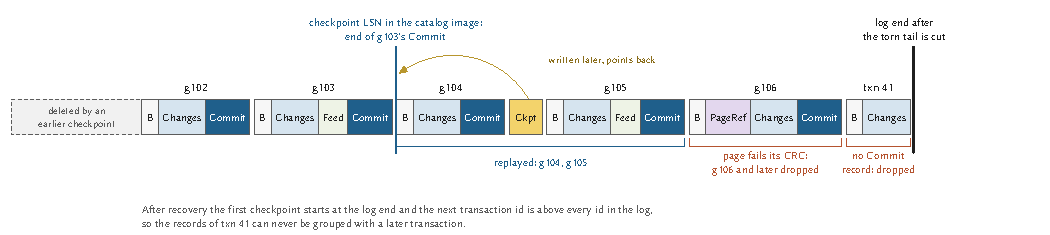
\includegraphics[width=\textwidth]{figures/wal}
\caption{Recovery reads the log from the checkpoint LSN recorded in the newest catalog image. It replays every commit whose \code{Commit} frame is valid, stops at the first commit whose referenced pages do not verify, and drops the records of transactions that never committed.}
\label{fig:wal}
\end{figure*}

\subsection{Recovery}
\label{sec:recovery}

Opening a database (\cref{fig:wal}) loads the newest valid catalog image, cuts the log's last segment at the end of its last valid frame, and reads the log from the image's checkpoint LSN. Records are grouped by transaction id. For each \code{Commit} frame in log order whose generation is newer than the image, recovery first restores the directory entries of the pages the commit references, then checks that every page referenced by a \code{PageRef} reads back with a valid header and the logged checksum, and then applies the commit's \code{Changes} to the trees of the previous generation. The replayed generations live in memory, exactly as they did before the crash, and the checkpoint that ends every open writes them.

Two rules make the recovered state a prefix of the commit order. First, a commit is part of the recovered state only if its \code{Commit} frame is in the log; records of transactions that never committed are dropped. Second, if one commit's pages fail verification, it and every later commit are dropped. The second rule matters after a power failure: the operating system may write the log to disk before the data pages it refers to, and a later commit's key changes apply to the trees of the commit before it, so replaying it on top of a lost commit would produce a state that never existed. Only commits that wrote pages can hit this rule, and none of them had been acknowledged, because acknowledgement comes after both syncs.

Recovery also guards against reusing what the log still holds. Transaction ids are persisted only in \code{Commit} records, so the id of a transaction that died during its commit would otherwise be handed out again while its records were still in the log, and a second crash would let recovery group the dead records with the new transaction's. Recovery therefore sets the next transaction id above every id it saw in the log, and the checkpoint at the end of the open starts from the end of the log rather than from the old checkpoint LSN, so those records are never read again.

Recovery writes nothing to the log, and the only state it leaves behind is published by the checkpoint at the end of the open, so a crash during recovery repeats the same work on the next open. History is not part of the catalog image. After a restart, time travel reaches the checkpointed generation and the generations replayed after it, and older states are available only through the change feed.
